
\newcommand{\insertTableTextSpace}{\vspace{0.0in}}

\newcommand{\insertTableRunTime}{
\begin{table}[t]
\begin{tabular}{c|c|c|c}
\toprule
%\getalloc{} for
\multirowcell{2}{Model \\ Update} & \multicolumn{3}{c}{\getalloc{} call time (s)} \\ \cline{2-4} 
 & \cilantrosw & \cilantroew & \cilantronjc\\
\midrule
%$0.0413 \pm 0.0048$ &  $2.8823 \pm 0.3155$ &  $2.1239 \pm 0.0212$ & $0.8132 \pm 0.162$ \\
$0.04 \pm 0.01$ &  $2.88 \pm 0.31$ &  $2.12 \pm 0.02$ & $0.81 \pm 0.16$ \\
\bottomrule
\end{tabular}
\vspace{0.05in}
\caption{\small
Mean time taken (in seconds) by \cilantro{} to update the performance model and for
computing a new allocation for each of the three fixed cluster sharing policies. 
% \insertTableTextSpace
% \insertTableTextSpace
\vspace{-0.3in}
}
\label{tab:mbtime}
\end{table}
}

\newcommand{\insertTableMetrics}{
\begin{table*}[t]
\centering
\begin{tabular}{c|c|c|c|c}
\toprule
Policy & Social Welfare, $(\socwel)$ & Egalitarian Welfare $(\egalwel)$ & NJC Fairness $(\njcfair)$
& Useful resource usage
 \\
\midrule
% ======== Data goes here =============
% Eurosys 2022 Data
% \oraclesw & $0.939 \pm 0.003$ & $0.315 \pm 0.010$ & $0.740 \pm 0.005$ & $0.961 \pm 0.002$ \\
% \oracleew & $0.825 \pm 0.004$ & $0.572 \pm 0.011$ & $0.706 \pm 0.002$ & $0.997 \pm 0.000$ \\
% \oraclenjc & $0.860 \pm 0.002$ & $0.482 \pm 0.010$ & $1.000 \pm 0.000$ & $0.991 \pm 0.000$ \\
% \midrule
% \cilantrosw & \textbf{0.910} $\pm$ \textbf{0.002} & $0.325 \pm 0.011$ & $0.739 \pm 0.010$ & $0.872 \pm 0.005$ \\
% \cilantroew & $0.811 \pm 0.004$ & \textbf{0.573} $\pm$ \textbf{0.012} & $0.740 \pm 0.010$ & $0.886 \pm 0.003$ \\
% \cilantronjc & $0.826 \pm 0.002$ & $0.492 \pm 0.005$ & \textbf{0.982} $\pm$ \textbf{0.006} * & \textbf{0.954} $\pm$ \textbf{0.003} \\
% \evoalgsw & $0.807 \pm 0.004$ & $0.209 \pm 0.009$ & $0.768 \pm 0.023$ & $0.761 \pm 0.006$ \\
% \evoalgew & $0.801 \pm 0.003$ & $0.220 \pm 0.008$ & $0.747 \pm 0.028$ & $0.777 \pm 0.005$ \\
% \equalshare & $0.667 \pm 0.002$ & $0.201 \pm 0.004$ & \textbf{1.000} $\pm$ \textbf{0.000} *
%     & $0.764 \pm 0.001$ \\
% \greedyew & $0.754 \pm 0.005$ & $0.287 \pm 0.003$ &  $0.90735 \pm 0.021$ & $0.807 \pm 0.003$ \\
% % \textcolor{red}{\greedyew} & $0.--- \pm 0.---$ & $0.--- \pm 0.---$ &  $0.--- \pm 0.---$ & $0.--- \pm 0.--$ \\

% \ernest & $0.753 \pm 0.003$ & $0.192 \pm 0.006$ & $0.865 \pm 0.012$ & $0.752 \pm 0.001$ \\
% \quasar & $0.833 \pm 0.002$ & $0.344 \pm 0.007$ & $0.747 \pm 0.006$ & $0.810 \pm 0.003$ \\
% \minerva & $0.733 \pm 0.030$ & $0.246 \pm 0.031$ & $0.609 \pm 0.002$ & $0.418 \pm 0.067$ \\

% NSDI 23 Data
\oraclesw & $0.892 \pm 0.004$ & $0.324 \pm 0.008$ & $0.336 \pm 0.004$ & $0.964 \pm 0.002$ \\
\oracleew & $0.752 \pm 0.003$ & $0.412 \pm 0.007$ & $0.272 \pm 0.002$ & $0.997 \pm 0.000$ \\
\oraclenjc & $0.828 \pm 0.002$ & $0.373 \pm 0.008$ & $0.999 \pm 0.000$ & $0.991 \pm 0.000$ \\
\midrule
\cilantrosw & \textbf{0.864} $\pm$ \textbf{0.006} & $0.337 \pm 0.013$ & $0.513 \pm 0.020$ & $0.818 \pm 0.012$ \\
\cilantroew & $0.760 \pm 0.007$ & \textbf{0.390} $\pm$ \textbf{0.020} & $0.426 \pm 0.037$ & \textbf{0.954} $\pm$ \textbf{0.012} \\
\cilantronjc & $0.823 \pm 0.002$ & $0.355 \pm 0.005$ & \textbf{0.964} $\pm$ \textbf{0.006} & $0.931 \pm 0.003$ \\
\evoalgsw & $0.649 \pm 0.017$ & $0.131 \pm 0.016$ & $0.182 \pm 0.048$ & $0.671 \pm 0.021$ \\
\evoalgew & $0.687 \pm 0.011$ & $0.158 \pm 0.012$ & $0.387 \pm 0.040$ & $0.700 \pm 0.009$ \\
\equalshare & $0.611 \pm 0.002$ & $0.151 \pm 0.006$ & \textbf{1.000} $\pm$ \textbf{0.000} & $0.766 \pm 0.001$ \\
\greedyew & $0.724 \pm 0.005$ & $0.306 \pm 0.006$ & $0.518 \pm 0.009$ & $0.882 \pm 0.004$ \\
\ernest & $0.675 \pm 0.002$ & $0.214 \pm 0.005$ & $0.891 \pm 0.013$ & $0.774 \pm 0.002$ \\
\quasar & $0.756 \pm 0.002$ & $0.095 \pm 0.003$ & $0.060 \pm 0.003$ & $0.706 \pm 0.002$ \\
\minerva & $0.555 \pm 0.017$ & $0.082 \pm 0.006$ & $0.034 \pm 0.005$ & $0.407 \pm 0.023$ \\
\parties & $0.661 \pm 0.002$ & $0.285 \pm 0.006$ & $0.645 \pm 0.000$ & $0.766 \pm 0.001$ \\
\AIMD & $0.761 \pm 0.002$ & $0.285 \pm 0.005$ & $0.745 \pm 0.000$ & $0.766 \pm 0.001$ \\
% ======== Data goes here =============
\bottomrule
\end{tabular}
\vspace{0.05in} 
\caption{\small
The social welfare~\eqref{eqn:socwel}, egalitarian welfare~\eqref{eqn:egalwel},
NJC fairness metric~\eqref{eqn:njcfair}, and the effective resource usage~\eqref{eqn:effresusage}
for all 13 methods.
Higher is better for all four metrics, and the maximum and minimum possible values for
all metrics are $1$ and $0$.
The values shown in bold have achieve the highest value for the specific metric, besides
the oracular policies.
\equalshare{} has NJC fairness $\njcfair=1$ by definition.
\insertTableTextSpace
\label{tab:metrics}
}
\end{table*}
}

\newcommand{\insertTableAS}{
\begin{table}[h]
\begin{tabular}{c|c|c}
\toprule
Policy & Performance & Cost \\
\midrule
\oracleas & $0.946 \pm 0.006$  & $134.528 \pm 2.555$ \\
\midrule
\cilantroas &  $0.940 \pm 0.006$  & $138.659 \pm 4.064$ \\
\kubeas & $0.903 \pm 0.010$  & $87.666 \pm 3.376$ \\
\pdas & $0.897 \pm 0.011$  & $86.771 \pm 3.303$ \\
\dstwo &  $0.951 \pm 0.010$  & $271.815 \pm 17.968$ \\
\midrule
\end{tabular}
\label{tab:autoscaling}
\caption{\small
Autoscaling experiment with Cilantro and baselines. Cilantro's performance is the closest to the specified threshold of 0.95 while minimizing cost.
}
\vspace{-2em}
\end{table}
}


\newcommand{\insertTableQueryBins}{
\begin{table}[t]
\centering
\begin{tabular}{c|c|c|c}
\toprule
Query Bin & TPC-DS Query Ids  & Mean Execution Time (s)\\
\midrule
\incmtt{db0} & 93, 91, 92, 45, 85, 15, 32 & 0.28
\\
\incmtt{db1} & 90, 84, 8, 55, 96, 81, 79 & 0.67
\\
% \incmtt{Bin 2} & 68, 62, 26, 71, 73, 66, 34 & 0.93
% \\
% \incmtt{Bin 3} & 76, 48, 13, 19, 12, 46, 7 & 1.24
% \\
% \incmtt{Bin 4} & 83, 44, 43, 3, 99, 41, 38 & 1.78
% \\
% \incmtt{Bin 5} & 20, 64, 61, 28, 65, 9, 31 & 4.02
% \\
% \incmtt{Bin 6} & 82, 52, 42, 74, 37, 40, 50 & 6.06
% \\
% \incmtt{Bin 7} & 98, 11, 29, 53, 89, 2, 33 & 7.27
% \\
% \incmtt{Bin 8} & 63, 88, 56, 25, 21, 95, 60 & 8.33
% \\
% \incmtt{Bin 9} & 59, 4, 57, 54, 49, 47, 78 & 18.22
% \\
\bottomrule
\end{tabular}
\vspace{0.05in}
\caption{\small Details of the bins created from TPC-DS queries. Each user's workload is generated using these bins. Execution time is profiled on a SQLite3 database running on AWS m5.2xlarge instance with one allocated CPU core.}
\label{tab:querybinmap}
\end{table}
}


\newcommand{\insertExpSetupTable}{
\begin{table}[]
\centering
\begin{tabular}{c|c|c|c}
\toprule
\textbf{Job and SLO Type}                              & \textbf{Job Name} & \textbf{SLO}  & \textbf{Utility Function} \\
\midrule
\multirow{10}{*}{Database Serving (Latency)}  & db01     & 0.9  & \incmtt{linear}           \\
                                              & db02     & 0.9  & \incmtt{linear}           \\
                                              & db03     & 0.95 & \incmtt{sqrt}             \\
                                              & db11     & 0.9  & \incmtt{linear}           \\
                                              & db12     & 0.9  & \incmtt{quadratic}        \\
                                              & db13     & 0.95 & \incmtt{quadratic}        \\
                                              & db14     & 0.95 & \incmtt{linear}           \\
                                              & db15     & 0.95 & \incmtt{quadratic}        \\
                                              & db16     & 0.99 & \incmtt{quadratic}        \\
                                              & db17     & 0.99 & \incmtt{sqrt}             \\
\midrule
\multirow{3}{*}{Prediction Serving (Latency)} & prs1     & 0.9  & \incmtt{linear}           \\
                                              & prs2     & 0.9  & \incmtt{sqrt}             \\
                                              & prs3     & 0.95 & \incmtt{sqrt}             \\
\midrule
\multirow{7}{*}{ML Training (Throughput)}     & mlt1     & 400  & \incmtt{sqrt}             \\
                                              & mlt2     & 400  & \incmtt{sqrt}             \\
                                              & mlt3     & 450  & \incmtt{linear}           \\
                                              & mlt4     & 450  & \incmtt{linear}           \\
                                              & mlt5     & 500  & \incmtt{quadratic}        \\
                                              & mlt6     & 500  & \incmtt{quadratic}        \\
                                              & mlt7     & 500  & \incmtt{quadratic}        \\
\bottomrule
\end{tabular}
\caption{\small
SLO and utility functions used for jobs in experiments in \S\ref{sec:fixedclus}. For Latency based SLOs, the SLO implies the fraction of queries that completed under 2 seconds. For Throughput based SLOs, the SLO is the desired query rate, measured in queries per second.
}
\label{tab:expjobsetup}
\end{table}
}


% \newcommand{\insertTableRelatedWork}{
% \begin{figure*}
% \centering
% 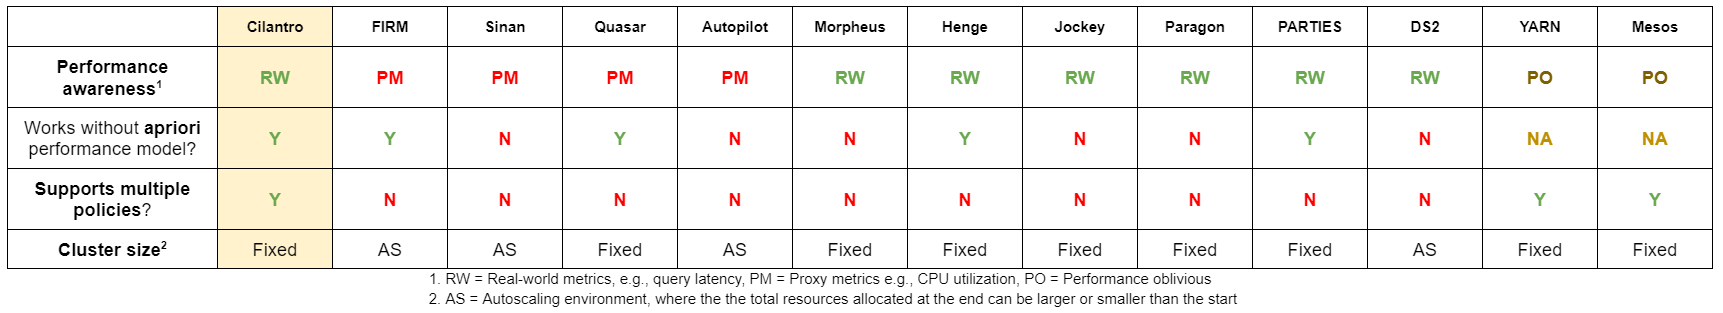
\includegraphics[width=\linewidth]{figs/Table.png}
% \vspace{-0.1in}
% \caption{\small
% Comparing Cilantro against related work. Cilantro \rbcomment{TODO - Make table in latex once approved. Create grouping RW PM PO. Move supports multiple policies to second.}
% \kkcomment{Supports multiple allocation objectives. Parties is not fixed cluster.}
% \label{tab:relatedworktable}
% \vspace{-0.1in}
% }
% \end{figure*}
% }

\newcommand{\rot}[1]{\makebox[2em][l]{\rotatebox{25}{\textbf{#1}}}}

\renewcommand\theadalign{cc}
\renewcommand\theadfont{\bfseries}
\renewcommand\theadgape{\Gape[1.2pt]}
\renewcommand\cellgape{\Gape[1.2pt]}

% How to generate this table:
% 1. Get source from https://docs.google.com/document/d/133x-sAJ_-8KBUKcCTZQIOdVTyAq881y9Mcu4AOdCQvw/edit
% 2. Paste in Excel
% 3. Paste in https://www.tablesgenerator.com/
\newcommand{\insertTableRelatedWork}{
\newcommand\colonewidth{1}
\newcommand\colschedwidth{2}
\begin{table*}[ht]
\small
\begin{threeparttable}
\begin{tabular}{p{1 cm}ccccccccccccc}
% ======= Copy only Tabular part from tablesgenerator.com, paste here. Add \makecell and \\ to create new line in text cells. Add citations and \rot to headers.==========
\multicolumn{1}{l}{}                                                      & \rot{Cilantro}                                                               & \rot{PARTIES\cite{chen2019parties}}                                        & \rot{Henge\cite{kalim2018henge}}                                          & \rot{Autopilot\cite{rzadca2020autopilot}}                                      & \rot{Jockey\cite{jockey}}                                         & \rot{Paragon\cite{delimitrou2013paragon}}                                        & \rot{Morpheus\cite{morpheus}}                                       & \rot{DS2\cite{kalavri2018three}}                                            & \rot{Quasar\cite{delimitrou2014quasar}}                                         & \rot{FIRM\cite{qiu2020firm}}                                           & \rot{Sinan\cite{zhang2021sinan}}                                          & \rot{YARN\cite{yarn}}                                           & \rot{Mesos\cite{mesos}}                                          \\ \hline
\multicolumn{1}{|c|}{\textbf{\makecell{Performance awareness}}}                      & \multicolumn{1}{c|}{\cellcolor[HTML]{FFF2CC}{\color[HTML]{6AA84F} \textbf{RW}}} & \multicolumn{1}{c|}{{\color[HTML]{6AA84F} \textbf{RW}}} & \multicolumn{1}{c|}{{\color[HTML]{6AA84F} \textbf{RW}}} & \multicolumn{1}{c|}{{\color[HTML]{6AA84F} \textbf{RW}}} & \multicolumn{1}{c|}{{\color[HTML]{6AA84F} \textbf{RW}}} & \multicolumn{1}{c|}{{\color[HTML]{6AA84F} \textbf{RW}}} & \multicolumn{1}{c|}{{\color[HTML]{6AA84F} \textbf{RW}}} & \multicolumn{1}{c|}{{\color[HTML]{6AA84F} \textbf{RW}}} & \multicolumn{1}{c|}{{\color[HTML]{FF0000} \textbf{PM}}} & \multicolumn{1}{c|}{{\color[HTML]{FF0000} \textbf{PM}}} & \multicolumn{1}{c|}{{\color[HTML]{FF0000} \textbf{PM}}} & \multicolumn{1}{c|}{{\color[HTML]{7F6000} \textbf{PO}}} & \multicolumn{1}{c|}{{\color[HTML]{7F6000} \textbf{PO}}} \\ \hline
\multicolumn{1}{|c|}{\textbf{\makecell{Works without apriori \\ performance model?}}} & \multicolumn{1}{c|}{\cellcolor[HTML]{FFF2CC}{\color[HTML]{6AA84F} \textbf{Y}}}  & \multicolumn{1}{c|}{{\color[HTML]{6AA84F} \textbf{Y}}}  & \multicolumn{1}{c|}{{\color[HTML]{6AA84F} \textbf{Y}}}  & \multicolumn{1}{c|}{{\color[HTML]{6AA84F} \textbf{Y}}}  & \multicolumn{1}{c|}{{\color[HTML]{FF0000} \textbf{N}}}  & \multicolumn{1}{c|}{{\color[HTML]{FF0000} \textbf{N}}}  & \multicolumn{1}{c|}{{\color[HTML]{FF0000} \textbf{N}}}  & \multicolumn{1}{c|}{{\color[HTML]{FF0000} \textbf{N}}}  & \multicolumn{1}{c|}{{\color[HTML]{6AA84F} \textbf{Y}}}  & \multicolumn{1}{c|}{{\color[HTML]{6AA84F} \textbf{Y}}}  & \multicolumn{1}{c|}{{\color[HTML]{FF0000} \textbf{N}}}  & \multicolumn{1}{c|}{{\color[HTML]{BF9000} \textbf{NA}}} & \multicolumn{1}{c|}{{\color[HTML]{BF9000} \textbf{NA}}} \\ \hline
\multicolumn{1}{|c|}{\textbf{\makecell{Supports multiple \\ allocation objectives?}}} & \multicolumn{1}{c|}{\cellcolor[HTML]{FFF2CC}{\color[HTML]{6AA84F} \textbf{Y}}}  & \multicolumn{1}{c|}{{\color[HTML]{FF0000} \textbf{N}}}  & \multicolumn{1}{c|}{{\color[HTML]{FF0000} \textbf{N}}}  & \multicolumn{1}{c|}{{\color[HTML]{FF0000} \textbf{N}}}  & \multicolumn{1}{c|}{{\color[HTML]{FF0000} \textbf{N}}}  & \multicolumn{1}{c|}{{\color[HTML]{FF0000} \textbf{N}}}  & \multicolumn{1}{c|}{{\color[HTML]{FF0000} \textbf{N}}}  & \multicolumn{1}{c|}{{\color[HTML]{FF0000} \textbf{N}}}  & \multicolumn{1}{c|}{{\color[HTML]{FF0000} \textbf{N}}}  & \multicolumn{1}{c|}{{\color[HTML]{FF0000} \textbf{N}}}  & \multicolumn{1}{c|}{{\color[HTML]{FF0000} \textbf{N}}}  & \multicolumn{1}{c|}{{\color[HTML]{6AA84F} \textbf{Y\textsuperscript{1}}}} & \multicolumn{1}{c|}{{\color[HTML]{6AA84F} \textbf{Y\textsuperscript{1}}}} \\ \hline
\multicolumn{1}{|c|}{\textbf{\makecell{Cluster size}}}                             & \multicolumn{1}{c|}{\cellcolor[HTML]{FFF2CC}Fix}                                & \multicolumn{1}{c|}{Var}                                & \multicolumn{1}{c|}{Fix}                                & \multicolumn{1}{c|}{Var}                                & \multicolumn{1}{c|}{Fix}                                & \multicolumn{1}{c|}{Fix}                                & \multicolumn{1}{c|}{Fix}                                & \multicolumn{1}{c|}{Var}                                & \multicolumn{1}{c|}{Fix}                                & \multicolumn{1}{c|}{Var}                                & \multicolumn{1}{c|}{Var}                                & \multicolumn{1}{c|}{Fix}                                & \multicolumn{1}{c|}{Fix}                                \\ \hline
% ======= Paste Done ==========
\end{tabular}
\begin{tablenotes}[flushleft]\footnotesize
\item abbr. RW = Real-world metrics, e.g., latency, PM = Proxy metrics e.g., CPU util., PO = Performance oblivious, Fix = Fixed size, Var = Variable size
\item [1] Supports multiple objectives, but only performance oblivious ones
\end{tablenotes}
\vspace{0.5em}
\vspace{-0.05in}
\caption{\small Cilantro and related work. Cilantro uses real-world metrics (e.g., latency) to build performance models online, which can be used to derive custom policies for different objectives.}
\vspace{-1em}
\label{tab:relatedwork}
\end{threeparttable}
\end{table*}
}
